\usepackage{lipsum}
\begin{document}

% =======================================================================================
%\cleardoublepage % Forces the first chapter to start on an odd page so it's on the right

% =======================================================================================
%                                   PREAMBLE
% =======================================================================================
\coverpage{\TITLE}{\SUBTITLE}{\AUTHOR}{\DATE}
%----------------------------------------------------------------------------------------
\newpage
\tableofcontents

% =======================================================================================
%                                   PART I
% =======================================================================================
\part{TÂCHE 1}
%----------------------------------------------------------------------------------------
\newpage
\chapter{ Compilation croisée et émulation ARM avec QEMU} \label{Compilation croisée et émulation ARM avec QEMU}
\section*{Introduction} \label{sec:Introduction}


Cette tâche vise à explorer la compilation croisée en utilisant un compilateur dédié à l'architecture ARM et à l'exécution de programmes ARM sur un système x86\_64 à l'aide de l'émulateur QEMU. En combinant ces deux technologies, nous permettons le développement et le test de logiciels ARM sur des plates-formes x86\_64, offrant ainsi une solution pratique pour le développement embarqué et la compatibilité multiplateforme. Ce projet offre un aperçu détaillé de la compilation croisée, de l'émulation d'architecture, et des outils nécessaires pour travailler efficacement dans un environnement ARM, même sur un système hôte x86\_64.



\section{Mise à jour des référentiels APT}
\begin{figure}[h]
  
    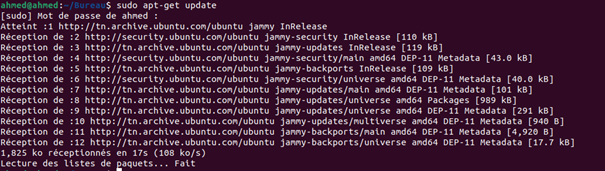
\includegraphics[width=1\textwidth]{images/Mise à jour des référentiels APT.png}
     
\end{figure}

\section{Installation des outils nécessaires, y compris le compilateur croisé pour ARM}

\begin{figure}[h]
  
    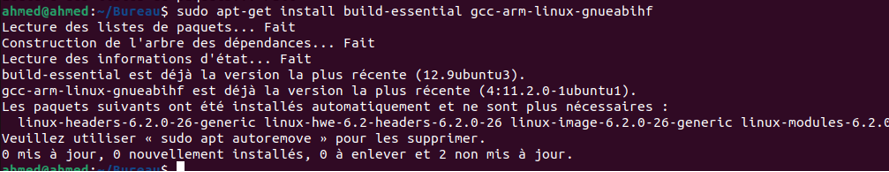
\includegraphics[width=1\textwidth]{images/outil.png}
   
\end{figure}

\section{Création d’un fichier hello.c  avec gedit}

\begin{figure}[h]

    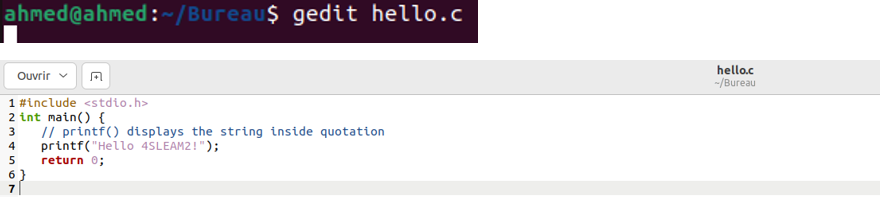
\includegraphics[width=0.8\textwidth]{images/1.png}

\end{figure}



\section{Compilation du fichier hello.c avec le compilateur croisé}

\begin{figure}[h]

    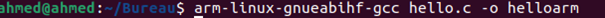
\includegraphics[width=1\textwidth]{images/2.png}

\end{figure}
\section{Installation de l'émulateur QEMU pour exécuter le binaire ARM}
\begin{figure}[h]

    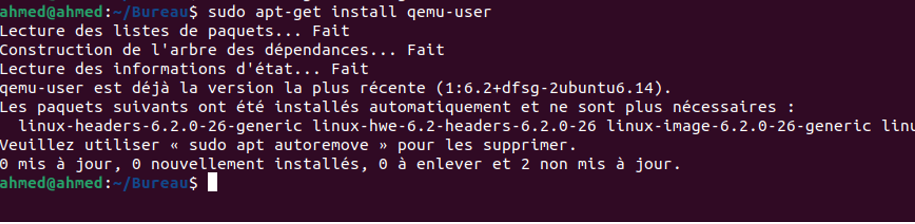
\includegraphics[width=1\textwidth]{images/3.png}

\end{figure}
QEMU (\textit{Quick EMUlator}) est un émulateur et un outil de virtualisation qui est souvent utilisé dans des projets tels que celui que vous avez décrit pour plusieurs raisons :
\begin{enumerate}
    \item \textbf{Émulation d'architecture :} QEMU est capable d'émuler différentes architectures matérielles, y compris l'architecture ARM. Cela signifie que vous pouvez exécuter des programmes destinés à ARM sur une machine x86\_64, ce qui est particulièrement utile pour le développement multiplateforme.
    \item \textbf{Facilité de configuration :} QEMU est relativement simple à installer et à configurer. Une fois que vous avez créé un environnement d'émulation ARM, il est facile d'y exécuter des binaires ARM sans avoir à déployer un matériel ARM réel.
    \item \textbf{Débogage :} QEMU offre des fonctionnalités de débogage puissantes, ce qui facilite le suivi et la résolution des problèmes dans les applications ARM sans avoir besoin d'un matériel ARM physique. Cela rend le développement et le test de logiciels plus pratiques.
    \item \textbf{Compatibilité :} QEMU est une solution bien établie et maintenue, ce qui signifie qu'elle est compatible avec de nombreuses distributions Linux et versions d'ARM, garantissant ainsi une grande flexibilité et une large base d'utilisateurs.
    \item \textbf{Performance raisonnable :} Bien que l'émulation soit généralement plus lente que l'exécution native, QEMU offre des performances suffisantes pour de nombreux cas d'utilisation de développement et de test, ce qui en fait un choix viable.
\end{enumerate}
\section{Création d’un lien symbolique pour le fichier ld-linux-armhf.so.3}
\begin{figure}[h]

    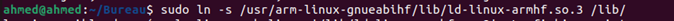
\includegraphics[width=1\textwidth]{images/4.png}

\end{figure}
On a créé un lien symbolique vers le fichier ld-linux-armhf.so.3 pour résoudre un problème de compatibilité d'architecture lors de l'exécution de programmes ARM sur une machine x86\_64 à l'aide de l'émulateur QEMU.

\section{Définir la variable LD\_LIBRARY\_PATH }
\begin{figure}[h]

    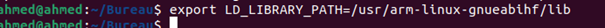
\includegraphics[width=1\textwidth]{images/5.png}

\end{figure}    
\section{Exécution du binaire ARM avec QEMU}
\begin{figure}[h]

    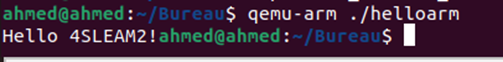
\includegraphics[width=0.8\textwidth]{images/7.png}

\end{figure}

\section{ Analyse du Fichier "helloarm" avec la Commande file}
\begin{figure}[h]

    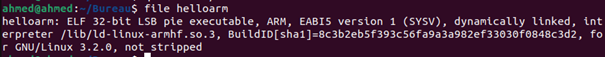
\includegraphics[width=1\textwidth]{images/6.png}

\end{figure}
La commande \texttt{file} permet d'obtenir des informations sur un fichier. Dans le cas de la commande \texttt{file helloarm}, elle retourne des informations sur le type de fichier, l'architecture cible, le système d'exploitation, etc.

Voici la décomposition des informations fournies :

\begin{itemize}
    \item \texttt{ELF 32-bit LSB ple executable} : Indique que le fichier est un fichier exécutable (ELF = Executable and Linkable Format) en 32 bits, utilisant un byte order (byte ordering) little-endian.
    \item \texttt{ARM, EABI version 1 (SYSV)} : Le fichier est conçu pour être exécuté sur une architecture ARM (Advanced RISC Machine), conformément à la version 1 de l'EABI (Embedded Application Binary Interface) et en utilisant le système d'exploitation SYSV (System V).
    \item \texttt{dynamically linked} : Le fichier contient des références à des bibliothèques externes, ce qui signifie qu'il faut d'abord charger ces bibliothèques pour exécuter le fichier.
    \item \texttt{interpreter /lib/ld-linux-armhf.so.3} : Le programme qui charge et exécute les dépendances dynamiques est /lib/ld-linux-armhf.so.3.
    \item \texttt{BuildID [sha1]=8c3b2eb5f393c56fa9a3a982ef33030f0848c3d2} : Un identifiant unique du fichier, calculé à l'aide de l'algorithme de hachage SHA-1.
    \item \texttt{for GNU/Linux 3.2.0} : Indique que le fichier a été compilé pour le système d'exploitation GNU/Linux, version 3.2.0.
    \item \texttt{not stripped} : Signifie que le fichier n'a pas été "strippé" (un processus qui supprime les informations de débogage pour réduire la taille du fichier et protéger le code source).
\end{itemize}

En somme, le fichier \texttt{helloarm} est un fichier exécutable en 32 bits pour une architecture ARM, compatible avec le système d'exploitation GNU/Linux 3.2.0 et utilisant l'EABI version 1 (SYSV). Il est compilé en utilisant le compilateur GNU/Linux.
\section*{Conclusion}
En conclusion, cette tâche "Cross-Compilation and ARM Emulation with QEMU" a permis d'explorer les concepts essentiels de la compilation croisée et de l'émulation d'architecture ARM sur des systèmes x86\_64. Grâce à l'utilisation d'un compilateur croisé, nous avons pu compiler des programmes spécifiques à l'architecture ARM sur un système hôte x86\_64. L'intégration de l'émulateur QEMU a ensuite permis d'exécuter ces programmes ARM avec succès, créant ainsi un environnement de test et de développement pratique pour les applications ARM.
%----------------------------------------------------------------------------------------


% =======================================================================================
%                                   PART II
% =======================================================================================

\part{TÂCHE 2}
\chapter{ Configuration d'un compilateur croisé } \label{ configuration d'un compilateur croisé en utilisant Crosstool-NG}
\section*{Introduction}
Ce rapport détaille le processus de configuration d'un compilateur croisé pour Raspberry Pi 3 (architecture aarch64) en utilisant Crosstool-NG, ainsi que la configuration de l'environnement pour l'utilisation du compilateur et la configuration de QEMU pour l'exécution de programmes compilés.
Crosstool-NG : Crosstool-NG est un outil de construction de chaînes de compilation croisée. Il est utilisé pour générer des outils de développement tels qu'un compilateur, un linker et d'autres utilitaires, spécifiquement conçus pour une architecture cible différente de celle du système de développement. Dans notre cas, nous utilisons Crosstool-NG pour construire un compilateur croisé pour l'architecture aarch64 (Raspberry Pi 3).
\section{Mise à jour du système }
Tout d'abord, nous avons mis à jour la liste des paquets disponibles et effectué une mise à niveau du système à l'aide des commandes suivantes :
\begin{itemize}
    \item sudo apt update
     \item sudo apt dist-upgrade
\end{itemize}
\section{Installation des dépendances}
Nous avons installé les dépendances nécessaires à la compilation en utilisant la commande :
\\sudo apt install build-essential git autoconf bison flex texinfo help2man gawk libtool-bin libncurses5-dev unzip 


\section{Clonage de Crosstool-NG }
Nous avons cloné le référentiel Crosstool-NG depuis GitHub en utilisant la commande :
\\git clone https://github.com/crosstool-ng/crosstool-ng 
\begin{figure}[h]
    \centering
    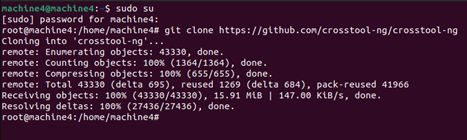
\includegraphics[width=1\textwidth]{images/8.png}
    
\end{figure}
\section{Accès au répertoire Crosstool-NG }
Nous nous sommes déplacés vers le répertoire nouvellement créé avec la commande :
\\cd crosstool-ng/ 
\begin{figure}[h]
    \centering
    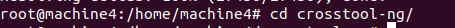
\includegraphics[width=1\textwidth]{images/9.png}
    
\end{figure}

\section{Bootstrap de Crosstool-NG }
Pour préparer l'environnement de compilation, nous avons exécuté la commande :
\\ ./bootstrap 
\section{Configuration de Crosstool-NG avec l'option --enable-local }
Nous avons configuré Crosstool-NG avec l'option --enable-local en utilisant la commande :
\\ ./configure --enable-local 
\begin{figure}[h]
    
    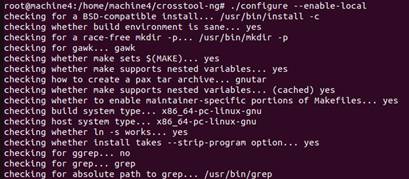
\includegraphics[width=1\textwidth]{images/10.png}   
\end{figure}
./configure --enable-local : La commande ./configure est couramment utilisée pour configurer un projet logiciel avant la compilation. Dans le cas de Crosstool-NG, ./configure --enable-local est utilisé pour configurer Crosstool-NG avec l'option --enable-local, qui indique à Crosstool-NG de construire la chaîne de compilation croisée localement, sur votre système. Cela signifie que la chaîne de compilation croisée sera générée sur votre système au lieu d'être téléchargée depuis des sources préconstruites.

\section{Compilation de Crosstool-NG }
Nous avons utilisé la commande \textbf{make} pour réellement construire Crosstool-NG, c'est-à-dire pour générer les outils de développement pour l'architecture cible.
\\Make est une commande de construction couramment utilisée dans les projets logiciels. Lorsqu'elle est exécutée, elle utilise un fichier Makefile pour compiler et assembler le code source du projet. 
\newpage
Dans le contexte de Crosstool-NG, make est utilisé pour réellement construire la chaîne de compilation croisée, c'est-à-dire pour générer les outils de développement pour l'architecture cible.
\begin{figure}[h]
    
    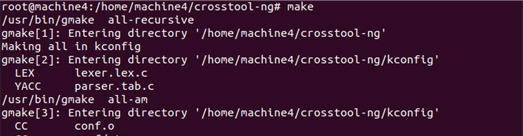
\includegraphics[width=1\textwidth]{images/11.png}   
\end{figure}

\section{Configuration de Crosstool-NG à l'aide de configurations prédéfinies}
Nous avons utilisé les configurations prédéfinies disponibles en utilisant la commande :

\textbf{./ct-ng list-samples }

\\ ./ct-ng list-samples est une commande qui liste les configurations prédéfinies (samples) disponibles pour Crosstool-NG. Ces configurations prédéfinies sont des ensembles de paramètres préconfigurés pour différentes architectures cibles. En utilisant cette commande, vous pouvez voir la liste des configurations prêtes à l'emploi pour choisir celle qui correspond à votre architecture cible.
\begin{figure}[h]
    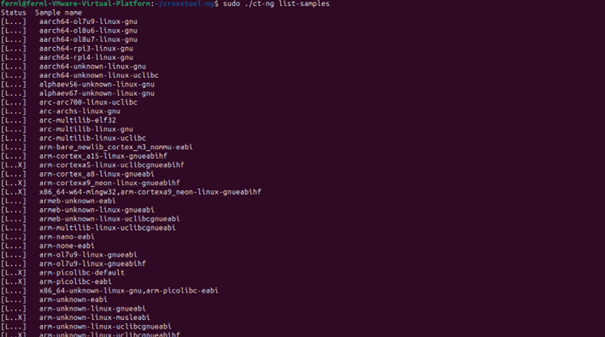
\includegraphics[width=1\textwidth]{images/12.png}   
\end{figure}

\section{Choix de la configuration prédéfinie }
Nous avons choisi la configuration prédéfinie pour l'architecture aarch64-rpi3-linux-gnu en utilisant la commande :
\\ ./ct-ng aarch64-rpi3-linux-gnu 
\newpage
\begin{figure}[h]
    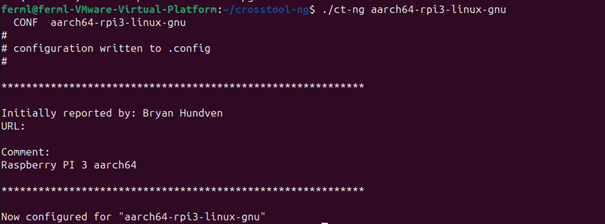
\includegraphics[width=1\textwidth]{images/13.png}   
\end{figure}
On peut utiliser ./ct-ng menuconfig pour configurer manuellement.  
\begin{figure}[h]
    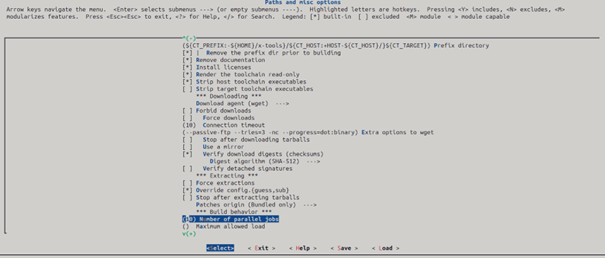
\includegraphics[width=1\textwidth]{images/14.png}   
\end{figure}
\section{Compilation du compilateur croisé}
 Nous avons lancé le processus de compilation du compilateur croisé en utilisant la commande :
\\ ./ct-ng build
\begin{figure}[h]
    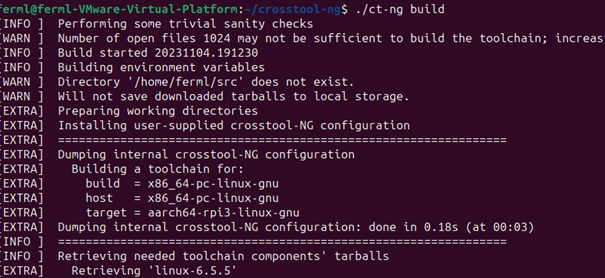
\includegraphics[width=1\textwidth]{images/15.png}   
\end{figure}

\section{Configuration de la variable PATH }
Nous avons configuré la variable PATH pour inclure le chemin du répertoire de notre compilateur croisé, tout en tenant compte de la configuration de LD\_LIBRARY\_PATH.
 Trouvez le chemin du répertoire où votre compilateur croisé a été installé. # Ajoutez le chemin du répertoire de votre compilateur croisé à la variable PATH en utilisant la commande suivante :
\begin{figure}[h]
    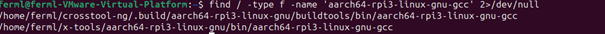
\includegraphics[width=1\textwidth]{images/16.png}   
\end{figure}

 \\export PATH=PATH:/home/ferml/x-tools/aarch64-rpi3-linux-gnu/bin
\begin{figure}[h]
    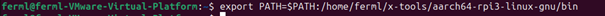
\includegraphics[width=1\textwidth]{images/17.png}   
\end{figure}

\section{Configuration de la variable CROSS\_COMPILE}
 Nous avons configuré la variable CROSS\_COMPILE dans les scripts de construction ou les fichiers de configuration pour spécifier le préfixe du compilateur croisé.
Trouvez le chemin du répertoire où votre compilateur croisé a été installé. # Configurez la variable CROSS\_COMPILE pour qu'elle corresponde au préfixe de votre compilateur croisé. export CROSS\_COMPILE=aarch64-rpi3-linux-gnu- 

\begin{figure}[h]
    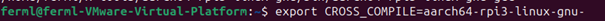
\includegraphics[width=1\textwidth]{images/19.png}   
\end{figure}
\section{Compilation d'un Programme de Test }
Une fois que vous avez créé avec succès la chaîne de compilation croisée avec Crosstool-NG, vous pouvez compiler un programme de test pour vérifier que le compilateur croisé fonctionne correctement. Assurez-vous d'avoir un fichier source, par exemple, testcompilation.c, que vous souhaitez compiler pour votre architecture cible.
\\Compilez le programme de test en utilisant le compilateur croisé que vous avez créé. Utilisez la commande aarch64-rpi3-linux-gnu-gcc (ou le préfixe approprié pour votre chaîne de compilation) pour compiler le programme. Par exemple :
\\aarch64-rpi3-linux-gnu-gcc -o testcompilation testcompilation.c 

\\Assurez-vous que testcompilation.c est le nom de votre fichier source et que vous spécifiez le nom de sortie (dans cet exemple, testcompilation).
\\Cette étape générera un exécutable pour votre architecture cible. 
\begin{figure}[h]
    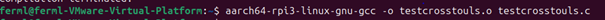
\includegraphics[width=1\textwidth]{images/20.png}   
\end{figure}

\section{Configuration de la variable LD\_LIBRARY\_PATH }
Nous avons configuré la variable LD\_LIBRARY\_PATH pour inclure le chemin des bibliothèques de notre compilateur croisé.
\\Configurez la variable LD\_LIBRARY\_PATH pour inclure 
\\le chemin des bibliothèques de votre compilateur croisé. 
\textbf{export LD\_LIBRARY\_PATH=/home/ferml/x-tools/aarch64-rpi3-linux-gnu/aarch64-rpi3-linux-gnu/sysroot/lib}


\section{Création d'un lien symbolique pour ld-linux-aarch64.so.1}
 Nous avons créé un lien symbolique pour `ld-linux-aarch64.so.1` pour assurer que le système cible peut trouver le linker dynamique nécessaire. ```bash # Créez un lien symbolique pour ld-linux-aarch64.so.1 dans le répertoire /lib du système. 
 \textbf{sudo ln -sf /home/ferml/x-tools/aarch64-rpi3-linux-gnu/aarch64-rpi3-linux-gnu/sysroot/lib/ld-linux-aarch64.so.1 /lib/ld-linux-aarch64.so.1 }
 \begin{figure}[h]
    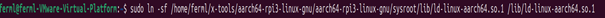
\includegraphics[width=1\textwidth]{images/21.png}   
\end{figure}
\section{Configuration de QEMU }
Pour exécuter des programmes compilés avec le compilateur croisé, nous avons configuré QEMU.
ferml@ferml-VMware-Virtual-Platform:~ aarch64-rpi3-linux-gnu-gcc -o testcompilation testcompilation.c
 \begin{figure}[h]
    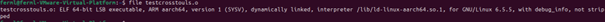
\includegraphics[width=1\textwidth]{images/22.png}   
\end{figure}
\\•	Assurez-vous que QEMU est installé avec la commande sudo apt install qemu.
\\•	Utilisez la commande qemu-aarch64 pour spécifier l'architecture cible.
 \begin{figure}[h]
    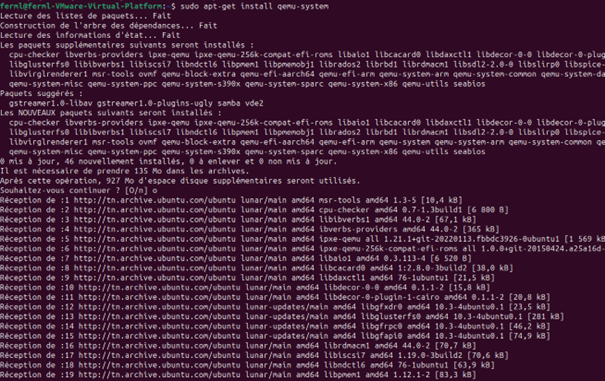
\includegraphics[width=1\textwidth]{images/23.png}   
\end{figure}
\newpage
\\ferml@ferml-VMware-Virtual-Platform:~ qemu-aarch64 ./testcompilation Hello, World!
 \begin{figure}[h]
    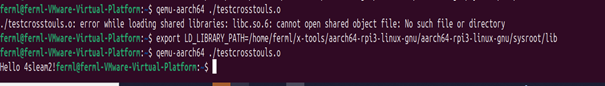
\includegraphics[width=1\textwidth]{images/24.png}   
\end{figure}

\section*{Conclusion}

En conclusion, ces étapes sont cruciales pour assurer le bon fonctionnement des programmes compilés avec le compilateur croisé sur le système cible, en particulier le Raspberry Pi 3. La configuration actuelle du système est désormais optimale pour le développement et les tests de logiciels spécifiquement adaptés à cette plateforme.

=======================================================================================
%                                   PART III
% =======================================================================================


\part{TÂCHE 3}
\chapter{ Création d'un appel système "Helloworld" } \label{  Création d'un nouveau module "Helloworld" }
\section*{Introduction}
Les appels système dans un système Linux embarqué sont des interfaces permettant aux applications d'interagir avec le noyau du système d'exploitation. Ils sont essentiels pour effectuer des opérations nécessitant des privilèges élevés ou un accès direct au matériel, généralement non autorisé pour les programmes utilisateur.

\textbf{Gestion des fichiers :}
\begin{itemize}
    \item \texttt{open() :} Pour ouvrir un fichier.
    \item \texttt{read() :} Pour lire à partir d'un fichier.
    \item \texttt{write() :} Pour écrire dans un fichier.
    \item \texttt{close() :} Pour fermer un fichier ou un descripteur de fichier.
\end{itemize}

\textbf{Gestion des processus :}
\begin{itemize}
    \item \texttt{fork() :} Pour créer un nouveau processus.
    \item \texttt{exec() :} Pour exécuter un nouveau programme dans le contexte du processus actuel.
    \item \texttt{wait() :} Pour attendre la fin d'un processus fils.
\end{itemize}

\textbf{Gestion des ressources système :}
\begin{itemize}
    \item \texttt{malloc() et free() :} Pour allouer et libérer de la mémoire dynamique.
    \item \texttt{brk() :} Pour ajuster la limite du segment de données.
\end{itemize}

\textbf{Gestion des fichiers et répertoires :}
\begin{itemize}
    \item \texttt{mkdir() :} Pour créer un répertoire.
    \item \texttt{rmdir() :} Pour supprimer un répertoire.
\end{itemize}

\textbf{Gestion des droits d'accès :}
\begin{itemize}
    \item \texttt{chmod() :} Pour modifier les permissions d'un fichier.
    \item \texttt{chown() :} Pour modifier le propriétaire d'un fichier.
\end{itemize}
\section{	Mise à jour du système}
sudo apt update && sudo apt upgrade
\section{	Installation des outils de développement}
sudo apt install gcc build-essential libncurses-dev libssl-dev libelf-dev bison flex -y
 \begin{figure}[h]
    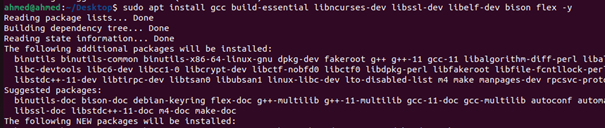
\includegraphics[width=1\textwidth]{images/25.png}   
\end{figure}
\section{Installation de l'outil "dwarves"}
sudo apt install dwarves
 \begin{figure}[h]
    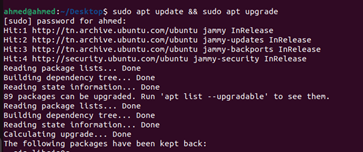
\includegraphics[width=1\textwidth]{images/26.png}   
\end{figure}
\section{	Nettoyage du système}
sudo apt clean && sudo apt autoremove -y
 \begin{figure}[h]
    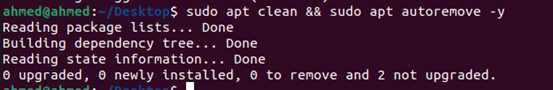
\includegraphics[width=1\textwidth]{images/27.png}   
\end{figure}
\section{	Téléchargement du noyau Linux 5.19.1}
wget -P ~/ https://mirrors.edge.kernel.org/pub/linux/kernel/v5.x/linux-5.19.1.tar.xz
 \begin{figure}[h]
    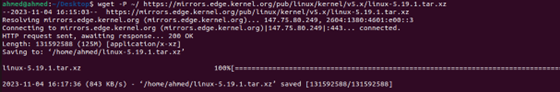
\includegraphics[width=1\textwidth]{images/28.png}   
\end{figure}
\section{Extraction des fichiers du noyau Linux 5.19.1}
tar -xvf ~/linux-5.19.1.tar.xz -C ~/
\section{Redémarrage système}
Rebbot
\section{Création d'un répertoire "helloworld" dans le répertoire "linux-5.19.1"}
cd linux-5.19.1
\\mkdir helloworld
\section{	Création du fichier "helloworld.c" dans le répertoire "helloworld"}
\begin{figure}[h]
    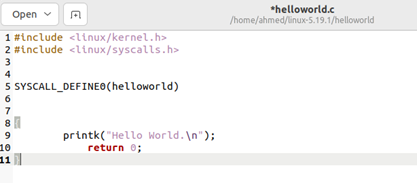
\includegraphics[width=1\textwidth]{images/29.png}   
\end{figure}
Le fichier \texttt{helloworld.c} contient un exemple de code pour créer un nouveau système d'appel (syscall) personnalisé dans le noyau Linux. Voici une explication détaillée de ce code :

\begin{itemize}
    \item Les fichiers d'en-tête \texttt{linux/kernel.h} et \texttt{linux/syscalls.h} sont inclus. Le premier contient des définitions et des structures utilisées par le noyau, tandis que le second contient des définitions et des structures spécifiques aux appels système.

    \item La fonction \texttt{SYSCALL\_DEFINE0(helloworld)} est définie. Cette macro est utilisée pour définir une nouvelle entrée de table de la table des appels système. La macro prend en argument le nom de la fonction et un ensemble d'arguments représentant les arguments passés à l'appel système.

    \item Le code suivant est simplement vide et est utilisé pour organiser le code.

    \item L'appel \texttt{printk("Hello World. \textbackslash n");} est utilisé pour afficher le message "Hello World." sur la console du système.

    \item Enfin, la fonction retourne 0, ce qui signifie que l'appel système s'est terminé avec succès.
\end{itemize}
\section{Création du fichire Makefile}
\begin{figure}[h]
    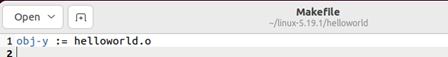
\includegraphics[width=1\textwidth]{images/30.png}   
\end{figure}
"obj-y := helloworld.o" dans un Makefile indique que le fichier objet "helloworld.o" doit être généré lors de la compilation du projet.

\section{Modification du fichier "Makefile}
\begin{figure}[h]
    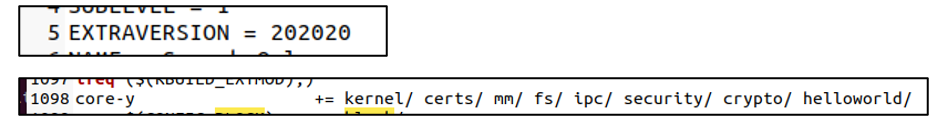
\includegraphics[width=1\textwidth]{images/31.png}   
\end{figure}
La modification du fichier "Makefile" en ajustant la variable d'extraversion et en ajoutant "helloworld" à la liste "core-y" après "block/" permet d'inclure le module "helloworld" dans la compilation du noyau Linux, tout en spécifiant la version du noyau cible, facilitant ainsi la personnalisation du noyau pour une configuration spécifique.
\section{Modification du fichier "syscalls.h" }
\begin{figure}[h]
    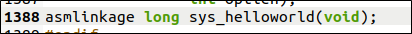
\includegraphics[width=1\textwidth]{images/32.png}   
\end{figure}
La modification du fichier "syscalls.h" pour ajouter une nouvelle déclaration de fonction système "sys\_helloworld" permet d'exposer une nouvelle fonction système dans le noyau Linux, que les programmes utilisateur peuvent appeler, étendant ainsi les fonctionnalités du noyau.
\section{Modification du fichier "syscall\_64.tbl}
\begin{figure}[h]
    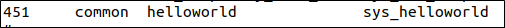
\includegraphics[width=1\textwidth]{images/33.png}   
\end{figure}
La modification du fichier "syscall\_64.tbl" pour ajouter l'entrée de la fonction système "sys\_helloworld" permet d'associer un numéro de syscall unique à cette nouvelle fonction système, permettant ainsi aux programmes utilisateur d'appeler la fonction "sys\_helloworld" de manière systématique en utilisant ce numéro de syscall spécifique. Cela garantit une interface cohérente pour accéder aux fonctionnalités ajoutées au noyau.
\newpage
\section{Configuration du noyau Linux en utilisant le menu de configuration}
sudo make menuconfig
\begin{figure}[h]
    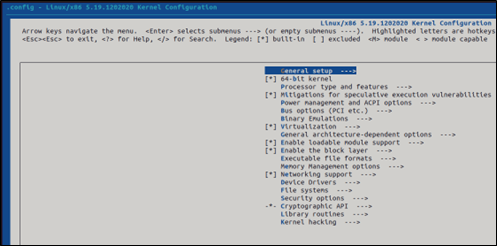
\includegraphics[width=1\textwidth]{images/34.png}   
\end{figure}
\section{Modification du fichier .conf}
\begin{figure}[h]
    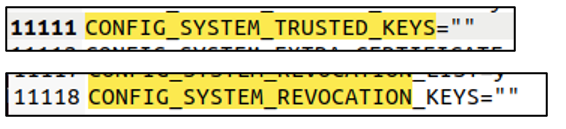
\includegraphics[width=1\textwidth]{images/35.png}   
\end{figure}
La modification du fichier de configuration du noyau Linux ("config") en supprimant le contenu entre les guillemets pour les options "CONFIG\_SYSTEM\_TRUSTED\_KEYS" et "CONFIG\_SYSTEM\_REVOCATIONS\_KEYS" signifie que l'on désactive la gestion des clés de confiance et des révocations du système, renforçant ainsi la sécurité du noyau en éliminant ces fonctionnalités potentiellement vulnérables.
\begin{figure}[h]
    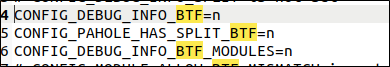
\includegraphics[width=1\textwidth]{images/36.png}   
\end{figure}
En changeant ces options de "y" à "n" dans la configuration du noyau Linux, vous désactivez la génération et l'utilisation de fichiers de débogage BTF (BPF Type Format). Cela réduit la taille de l'image du noyau et peut améliorer les performances, mais cela signifie que certaines fonctionnalités de débogage BTF ne seront pas disponibles, ce qui peut rendre le débogage plus difficile. Cette modification est généralement effectuée pour optimiser la configuration du noyau pour des scénarios spécifiques, comme les systèmes embarqués où l'espace disque est limité.
\section{Affichage du nombre de processeurs}
\begin{figure}[h]
    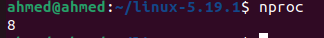
\includegraphics[width=0.7\textwidth]{images/37.png}   
\end{figure}
\section{Compilation du noyau}
\textbf{sudo make -j8}

\\La commande "make" est utilisée pour compiler et construire le noyau Linux, ainsi que d'autres composants du système. L'option "-j8" indique le nombre de tâches parallèles à exécuter lors de la compilation (8 dans cet exemple). En résumé, "make" est essentiel pour générer les binaires et les fichiers système nécessaires au fonctionnement du système embarqué Linux.
\section{18-	Installation des modules du noyau Linux }
\textbf{sudo make modules\_install -j8}
\begin{figure}[h]
    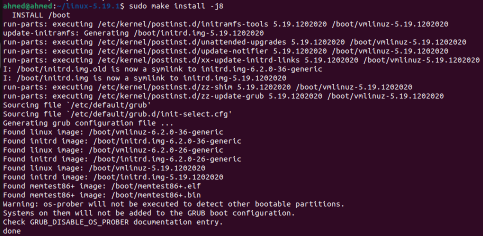
\includegraphics[width=1\textwidth]{images/39.png}   
\end{figure}

\section{Modification du fichier GRUB }
La configuration du fichier GRUB a été modifiée en passant du mode d'affichage automatique à un menu avec un délai de 10 secondes, permettant une sélection plus souple du noyau Linux au démarrage.
\newpage
\begin{figure}[h]
    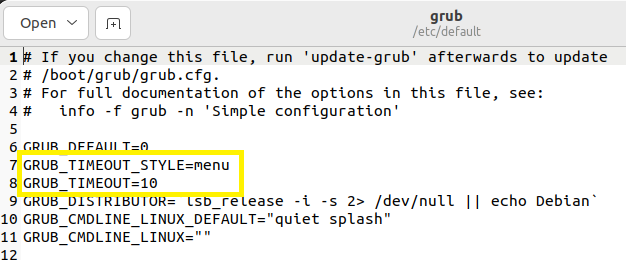
\includegraphics[width=0.8\textwidth]{images/40.png}   
\end{figure}
\section{Mise à jour du gestionnaire de démarrage GRUB }
\textbf{sudo update-grub}
\begin{figure}[h]
    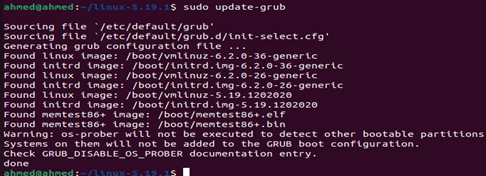
\includegraphics[width=0.8\textwidth]{images/41.png}   
\end{figure}

\section{Redémarrage du système pour démarrer avec le nouveau noyau Linux}
\begin{figure}[h]
    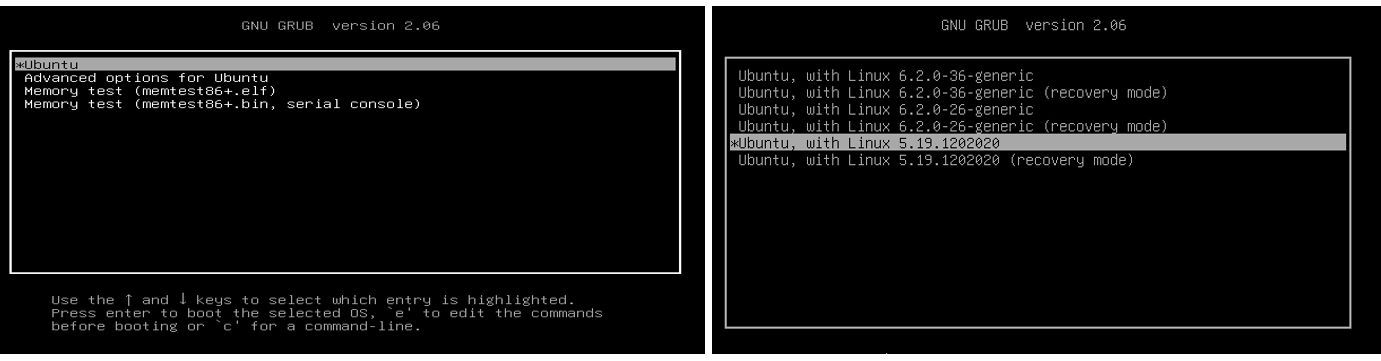
\includegraphics[width=0.8\textwidth]{images/42.png}   
\end{figure}

\section{Création du fichier testapellesystem }
\begin{figure}[h]
    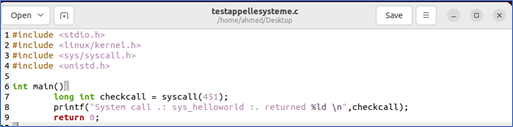
\includegraphics[width=0.8\textwidth]{images/43.png}   
\end{figure}
Ce programme est conçu pour appeler un appel système personnalisé (nommé "sys\_helloworld") et afficher le résultat de cet appel sur la sortie standard. La valeur renvoyée par l'appel système peut être utilisée pour communiquer des informations entre le noyau et l'application utilisateur.

\section{Compilation du programme C "testappellesysteme.c" }
\begin{figure}[h]
    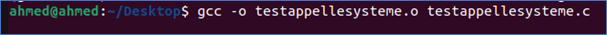
\includegraphics[width=0.8\textwidth]{images/44.png}   
\end{figure}
\section{Exécution du programme "testappellesysteme.o" }
\begin{figure}[h]
    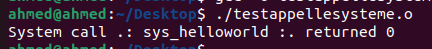
\includegraphics[width=0.8\textwidth]{images/45.png}   
\end{figure}

\section{Exécution de la commande dmesg pour afficher les messages du noyau}
\begin{figure}[h]
    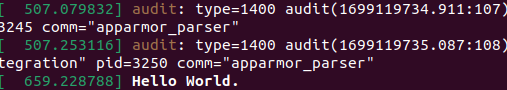
\includegraphics[width=0.8\textwidth]{images/46.png}   
\end{figure}

La commande dmesg est utilisée dans les systèmes d'exploitation de type Unix, y compris Linux, pour afficher les messages du noyau du système. Le nom "dmesg" signifie "display message" (afficher les messages). Cette commande permet d'examiner les messages générés par le noyau Linux pendant le processus de démarrage du système et fournit des informations sur les événements du noyau, les erreurs, les avertissements et d'autres activités liées au matériel.

\section*{Conclusion}
Cette tache a s’agit  d’un processus complet de création d'un module de noyau Linux nommé "helloworld". Les étapes comprenaient l'installation d'outils, le téléchargement d'une version du noyau Linux, la configuration du noyau pour ajouter un nouveau module, la modification de fichiers sources, la compilation du noyau, et l'exécution d'un programme utilisateur qui appelait la nouvelle fonction système. En fin de compte, ce projet  permet de mieux comprendre les bases de la création de modules de noyau, de la configuration du noyau, de l'appel de fonctions système depuis des programmes utilisateur, de la compilation et de l'installation d'un noyau personnalisé.

=======================================================================================
%                                   PART 4
% =======================================================================================

\part{TÂCHE 4}
\chapter{ Création d'un module de noyau} \label{ Création d'un module de noyau}
\section*{Introduction}
Le développement de modules de noyau sous Linux offre une puissante méthode pour étendre ou personnaliser le comportement du noyau. Un module de noyau est un programme qui peut être dynamiquement chargé et déchargé dans le noyau du système d'exploitation sans nécessiter de redémarrage. Ces modules fournissent une manière flexible d'ajouter des fonctionnalités au noyau sans avoir à recompiler l'ensemble du noyau ou à modifier le code source du noyau directement.
\section{Installation des package nécessaires}
\textbf{sudo apt-get install build-essential linux-headers-(uname -r)}
\section{Création du répertoire du module}
\textbf{mkdir kernel\_modules}
\\\textbf{cd kernel\_modules}
\section{Création du fichier source du module}
\begin{figure}[h]
    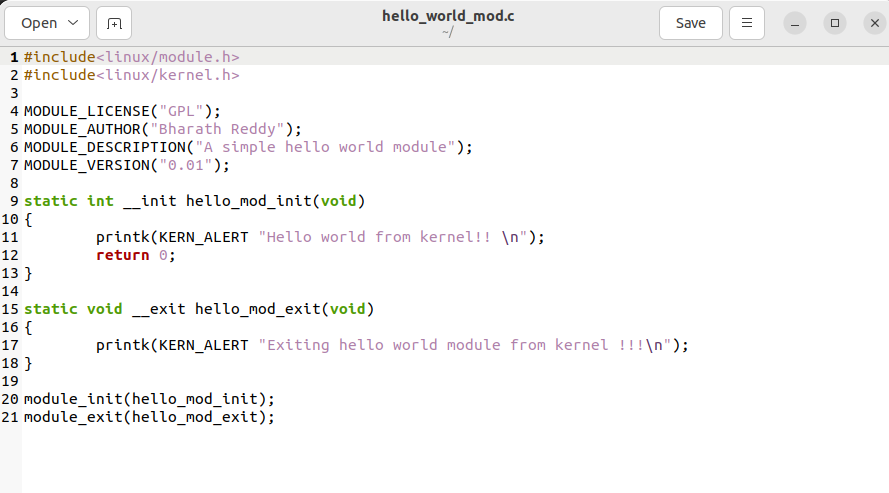
\includegraphics[width=0.8\textwidth]{images/47.png}   
\end{figure}

Ce code crée un module de noyau simple qui, lorsqu'il est chargé, écrit "Hello world from kernel!!" dans les logs du noyau, et lorsqu'il est déchargé, écrit "Exiting hello world module from kernel !!!"

\section{Création du fichier Makefile}

Le fichier Makefile dans le contexte du développement de modules de noyau sous Linux est un script utilisé par l'utilitaire make pour automatiser le processus de compilation. Son rôle est de spécifier comment les fichiers source doivent être compilés et liés pour créer le module de noyau.
\begin{figure}[h]
    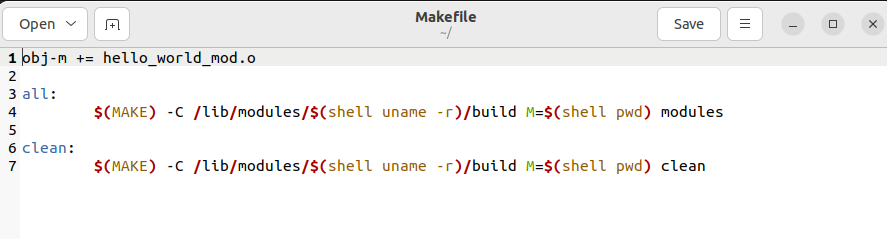
\includegraphics[width=0.8\textwidth]{images/48.png}   
\end{figure}
\\Ce fichier est conçu pour être utilisé avec le système de construction du noyau Linux. La cible all compile le module, tandis que la cible clean supprime les fichiers temporaires générés lors de la compilation. Ces commandes simplifient le processus de compilation et de nettoyage des modules du noyau.
\section{Compilation du module}
\textbf{make all}
\begin{figure}[h]
    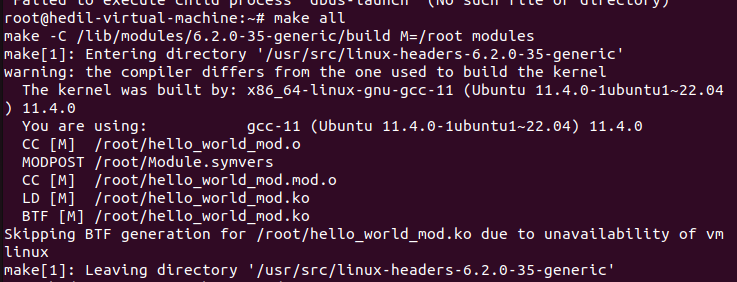
\includegraphics[width=0.8\textwidth]{images/49.png}   
\end{figure}

\section{Chargerment du module}
\begin{figure}[h]
    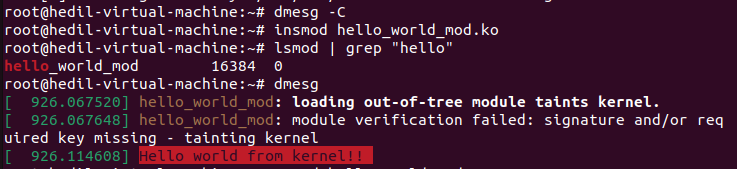
\includegraphics[width=0.8\textwidth]{images/50.png}   
\end{figure}
\newpage
\textbf{1- Réinitialisation du tampon des messages du noyau}
\\dmesg -c

\\\textbf{2- Chargerment du module}
\\sudo insmod hello\_world\_mod.ko

\textbf{3- Vérifier le chargement du module}
\\lsmod | grep "hello"

\\\textbf{4- Vérifier les journaux système (dmesg) }
\\dmesg

\section{Déchargerment du module}

\begin{figure}[h]
    \includegraphics[width=0.8\textwidth]{images/51.png}   
\end{figure}


\\\textbf{1- Déhargerment du module}
\\sudo rmod hello\_world\_mod.ko


\\\textbf{2- Vérifier les journaux système (dmesg) }
\\dmesg

\section*{Conclusion}
Cette tâche a démontré les concepts fondamentaux du développement de modules de noyau, offrant un aperçu de la manière dont ces modules peuvent être utilisés pour étendre la fonctionnalité du noyau Linux de manière dynamique et flexible. Elle constitue une base solide pour des projets plus avancés impliquant des modules de noyau personnalisés.











\end{document}
